\section{Resultados} \label{sec:result}
\subsection{Planejamento do experimento} \label{subsec:planexp}

Na fase inicial desse estudo diversos experimentos numéricos realizados  sugeriram que sistemas desequilibrados podiam ser representados usando-se sistemas equilibrados equivalentes em certo sentido específico, com um erro que que podia ser estimado a priori. 
    
Então foi planejado e executado um experimento numérico para testar a seguinte hipótese: O \textit{makespan} de sistemas de manufatura com $m$ máquinas e $n$ lotes com tempos distintos $p_i$ de processamento em cada máquina $i$ podem ser estimados adequadamente usando-se um tempo médio $p$ para cada máquina?

Deste modo, o planejamento do experimento foi baseado na geração de cenários aleatórios de sistemas produtivos a fim de realizar simulações. O planejamento então seguiu as seguintes etapas:

\begin{itemize}
    \item Geração dos dados do problema (cenários);
    \item Modelagem do problema no \textit{Software R};
    \item Execução das simulações utilizando dados os cenários gerados e geração dos resultados;
    \item Análise os resultados das simulações.
\end{itemize}


    \subsubsection{Geração dos dados}
    
    Na literatura, a teoria para as técnicas de \textit{Lot Streaming} com sistemas de 2 e 3 máquinas já estão bem consolidadas, portanto o experimento buscou simular cenários com 5, 10 e 15 máquinas, a fim de ter uma visão mais geral do problema, uma vez que os problemas mais gerais (de $m$ máquinas) podem ser resolvidos em $m-1$ subproblemas de pares de máquinas. Além de variar o número de máquinas ($m$), o tempo de processamento das máquinas ($p$) variou em até 20\%, 50\% e 70\% entre os pares de máquinas, de modo que permitisse observar a diferença entre sistemas mais equilibrados e menos equilibrados. 
    
    Portanto, foram gerados 9 grupos de cenários aleatórios, sendo eles cenários com:
    \begin{itemize}
        \item 5 máquinas com variação até 20\%;
        \item 5 máquinas com variação até 50\%;
        \item 5 máquinas com variação até 70\%;
        \item 10 máquinas com variação até 20\%;
        \item 10 máquinas com variação até 50\%;
        \item 10 máquinas com variação até 70\%;
        \item 15 máquinas com variação até 20\%;
        \item 15 máquinas com variação até 50\%;
        \item 15 máquinas com variação até 70\%.
    \end{itemize}
    
    Os tempos de máquinas de cada cenários foram gerados de maneira aleatória seguindo as condições de variação correspondentes. Os tempos de processamento de cada máquina foi gerado da seguinte maneira: o tempo de processamento da máquina $m_1$ ($p_1$) foi obtido de uma distribuição normal de média 9 com desvio padrão de 3. Para $p_2$, utilizou-se o tempo $p_1$ e definiu uma variação de até 20, 50 ou 70\% para mais ou para menos de acordo com a restrição do conjunto. O processo se repete até $p_m$ (tempo de processamento da máquina $m$).
    
    Em relação à quantidade de itens a serem processadas ($U$), o valor de 2000 unidades foi escolhido, uma vez que o número de sublotes ($n$) a serem divididos foi de 1 a 6, sendo que a partir de 6 sublotes o ganho no \textit{makespan} passa a ser menor que 5\%. 
    
    Já para os cenários equilibrados equivalentes, foi calculado o tempo apenas de uma máquina ao qual replicou-se para as demais, uma vez que todos os tempos são iguais. Tendo os tempos do cenário desequilibrado $p_1$, $p_2$, $p_3$, \ldots, $p_m$, calcula-se uma taxa de tempo médio ($tx$) dado pela Equação~\ref{eq:txtempo}.
    
    \begin{eqnarray}
        tx = \frac{p_1+2p_2+2p_3+\ldots+p_m}{m-1}
        \label{eq:txtempo}
    \end{eqnarray}
    
    Como o cenário equilibrado equivalente tem todos os tempos de processamento iguais, então $p_1=p_2=p_1=p_3=\ldots=p_m$, chamando o tempo de processamento do cenário equilibrado de $p_{eq}$, então temos a Equação~\ref{eq:txtempoeq}.
    
    \begin{eqnarray}
        tx = \frac{p_{eq}+2p_{eq}+2p_{eq}+\ldots+p_{eq}}{m-1}
           = \frac{(2m-2)p_{eq}}{m-1}
        \label{eq:txtempoeq}
    \end{eqnarray}
    
    Logo, chegamos a Equação~\ref{eq:peq} para obtenção do tempo das máquinas do sistema equilibrado equivalente.
    
    \begin{eqnarray}
        p_{eq}=\frac{tx}{2}
        \label{eq:peq}
    \end{eqnarray}
    
    Com os dados gerados, seguindo a Simulação de Monte Carlo, cada conjunto de cenários foram replicados 100 vezes. Vide Apêndices~\ref{app:tab05machine20},~\ref{app:tab05machine50},~\ref{app:tab05machine70},~\ref{app:tab10machine20},~\ref{app:tab10machine50},~\ref{app:tab10machine70},~\ref{app:tab15machine20},~\ref{app:tab15machine50} e~\ref{app:tab15machine70} com todos os cenários gerados.
    
    
    \subsubsection{Modelagem do problema}
    
    A modelagem do problema se deu a partir do uso do \textit{Software R} como ferramenta para modelagem e execução das simulações.
    
    Utilizando-se dos dados gerados pelas simulações e seguindo as premissas das técnicas de \textit{Lot Streaming}, foi possível modelar um sistema de produção com máquinas processando em série, de modo que permitisse também o processamento em sobreposição de alguns itens. 
    
    Nas técnicas de \textit{Lot Streaming} para se obter o valor do \textit{Makespan}, é preciso além dos dados do sistema, calcula a quantidade de sublotes ($n$) e o tamanho dos sublotes ($L$). 
    
    É importante ressaltar que pelo fato de não existir uma teoria geral para o problema geral de \textit{lot streaming}, os cálculos utilizados são para problemas de 2 máquinas, uma vez que o experimento se deu por meio da resolução de $m-1$ subproblemas de 2 máquinas.
    
    A teoria estabelecida para o problema de 2 máquinas, afirma que deve-se determinar o número de sublotes a serem divididos, onde $U = L _ { 1 } + L _ { 2 } + \ldots + L _ { n }$. Para o experimento foram simulados começando com 1 sublote (isto é, sem o \textit{Lot Streaming}) até 6 sublotes, uma vez que foi observado que a partir dessa quantidade os ganhos no \textit{Makespan} foram inferiores a 5\%.
    
    Ainda, de acordo com \citeonline{Trietsch1993}, os tamanhos de sublotes devem seguir uma progressão geométrica dada pela Equação~\ref{eq:tamanhosublote}. 
    
    \begin{eqnarray}
        L _ { j } = q L _ { j - 1 } = q ^ { j - 1 } L _ { 1 }
        \label{eq:tamanhosublote}
    \end{eqnarray}
    
    Onde, $q$ é a razão $p_2/p_1$ (no caso de 2 máquinas).
    
    Como o objetivo é de abranger um caso mais geral o sistema é caracterizado como uma sistema de tamanho de sublotes variáveis, isto é, para cada subproblema de 2 máquinas o tamanho de sublotes é diferente, conforme o exemplo da Figura~\ref{fig:LS_ex3}. Ainda, o sistema permite a ociosidade intermitente entre máquinas, entretanto os tamanhos de sublotes é representado de maneira discreta para fins de possível aplicação prática. 
    
    Para calcular o \textit{Makespan} (denotado por $M$) foi necessário simular cada subproblema de 2 máquinas, uma vez que o trabalho trata de um problema discreto e não há uma fórmula geral para calcular esse tempo de completude nesta situação, apenas para problemas contínuos.
    
    Além disso, também foi calculado o \textit{Makespan} dos cenários equilibrados equivalente, denotado por $M_{eq}$.
    
    Por fim, para cada cenário foi calculado o \textit{Makespan} partindo de 1 sublote à 6 sublotes, da mesma maneira para os cenários equilibrados equivalentes. Tendo ambos resultados em mãos, calcula-se então o desvio gerado pela diferença de desempenho do cenário desequilibrado para o seu equivalente. No decorrer deste trabalho este desvio será chamado de erro ($e$), e é calculado conforme a Equação~\ref{eq:erromakespan}.
    
    \begin{eqnarray}
        e = \left|\frac{M - M_{eq}}{M_{eq}}\right|
        \label{eq:erromakespan}
    \end{eqnarray}
    
    
    \subsubsection{Resultados gerados pelas simulações}
    
    Rodando, portanto, o programa para cada um dos conjuntos de cenários foi obtido os resultados do \textit{Makespan}, tanto para equilibrado quanto desequilibrado, bem como o erro gerado entre esses tempos de completude. 
    
    Na Figura~\ref{fig:M05_20}, é possível observar o comportamento do \textit{Makespan} de todos os cenários do conjunto com 5 máquinas e variação de até 20\%. A Figura~\ref{fig:Meq05_20} é referente aos cenários equilibrados equivalentes deste conjunto. Cada linha dos gráficos representa o \textit{Makespan} de um cenário e mostra como ele vai reduzindo conforme aumenta-se o número de sublotes. Para uma melhor visualização, no Apêndice~\ref{app:fig05machine20}, estão os gráficos dos cenários junto aos seus equivalentes, sendo as Figuras~\ref{fig:05m20_01-10} a~\ref{fig:05m20_91-100}. Também, na Figura~\ref{fig:e05_20} são representados os erros gerados a partir da Equação~\ref{eq:erromakespan}, como já mencionado. 
    
    %% 5 Machine 20%
    \begin{figure}[!ht]
    \centering
    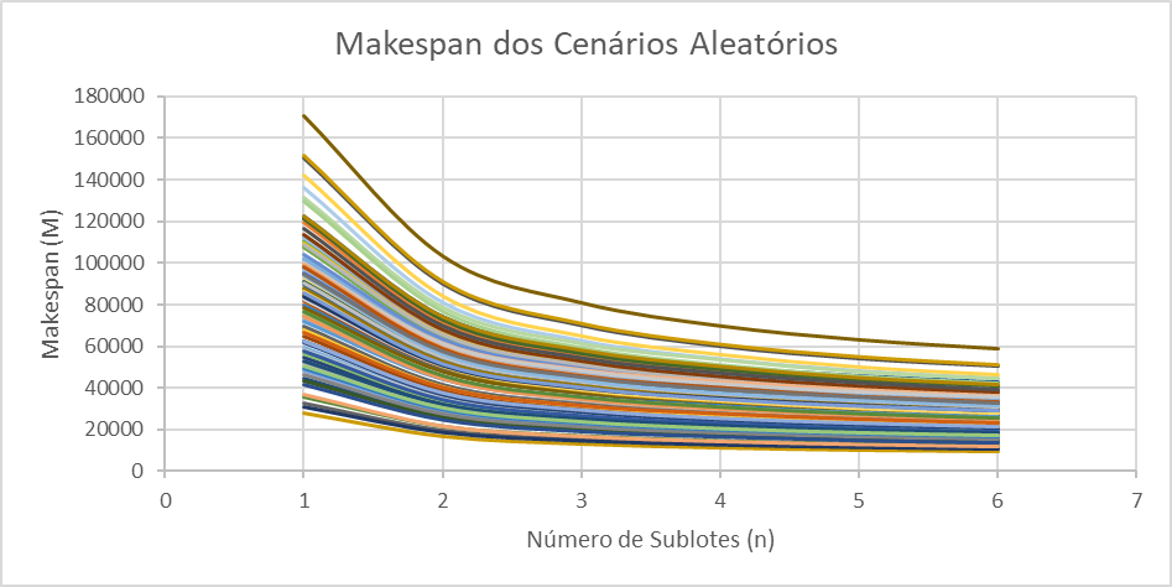
\includegraphics[width=12cm]{Resultados/Figuras/M05_20}
    \caption{Makespan dos cenários com 5 máquinas e variação de até 20\%}
    \label{fig:M05_20}
\end{figure}
    
    \begin{figure}[!ht]
    \centering
    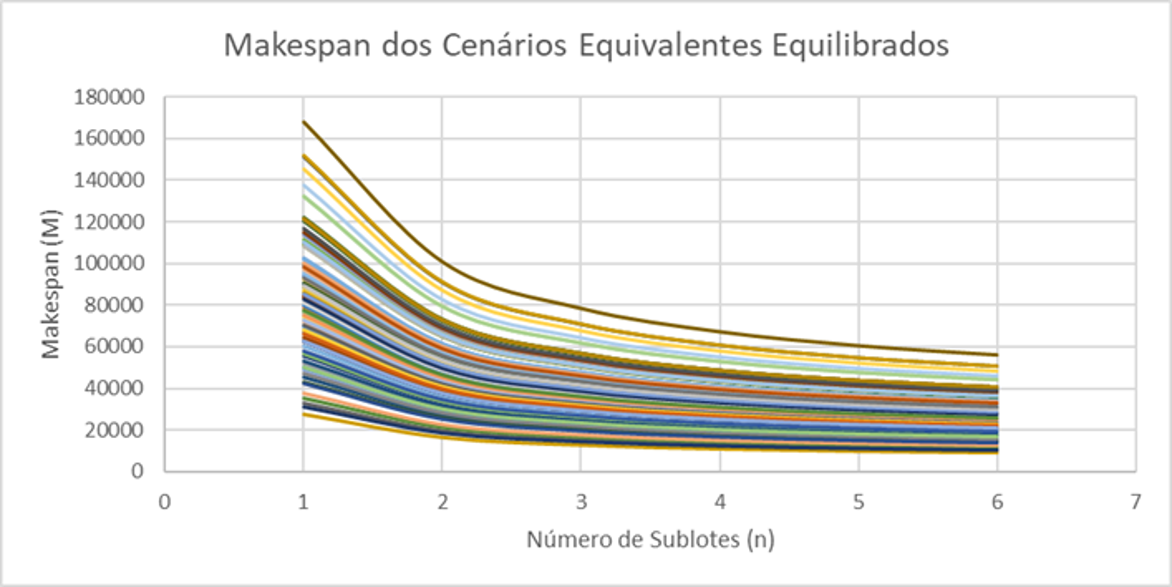
\includegraphics[width=12cm]{Resultados/Figuras/Meq05_20}
    \caption{Makespan dos cenários equilibrados equivalentes com 5 máquinas e variação de até 20\%}
    \label{fig:Meq05_20}
\end{figure}
    
    \begin{figure}[!ht]
    \centering
    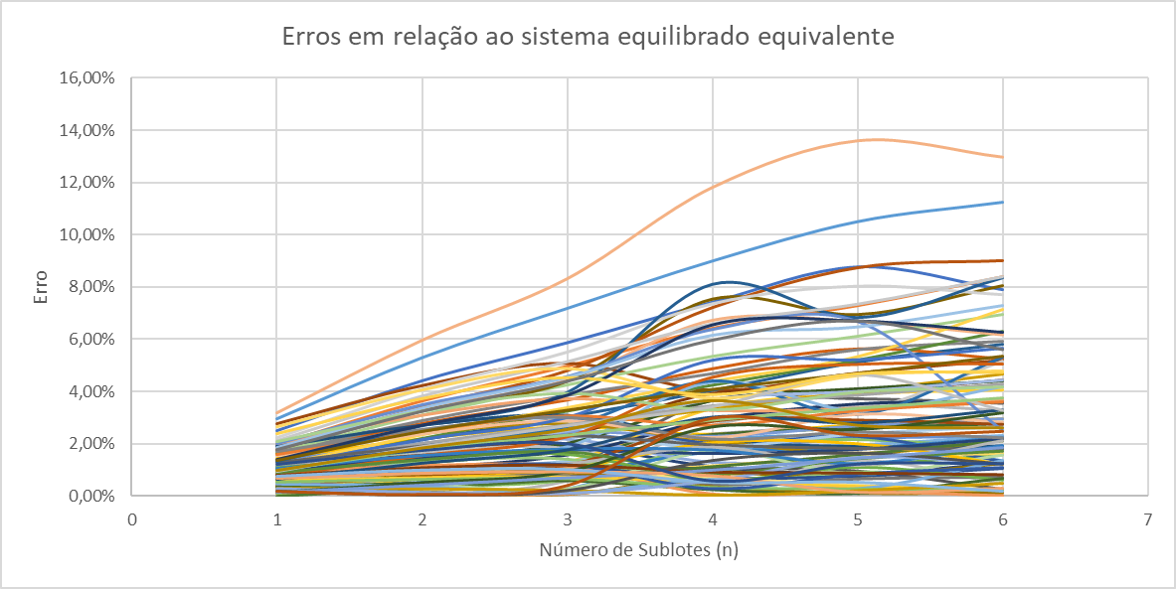
\includegraphics[width=12cm]{Resultados/Figuras/e05_20}
    \caption{Erros dos cenários com 5 máquinas e variação de até 20\%}
    \label{fig:e05_20}
\end{figure}
    
    Para o conjunto de 5 máquinas e até 50\% de variação entre pares de máquinas tem-se as Figuras~\ref{fig:M05_50} e~\ref{fig:Meq05_50} representando respectivamente o \textit{Makespan} dos cenários aleatórios e os cenários equilibrados equivalentes. A Figura~\ref{fig:e05_50} mostra os erros dos cenários desse conjunto. Seguindo a mesma representação do conjunto anterior, no Apêndice~\ref{app:fig05machine50} encontram-se os gráficos comparativos com os cenários detalhados com seus equivalentes (Figuras~\ref{fig:05m50_01-10} a~\ref{fig:05m50_91-100}).
    
    %% 5 Machine 50%
    \begin{figure}[!ht]
    \centering
    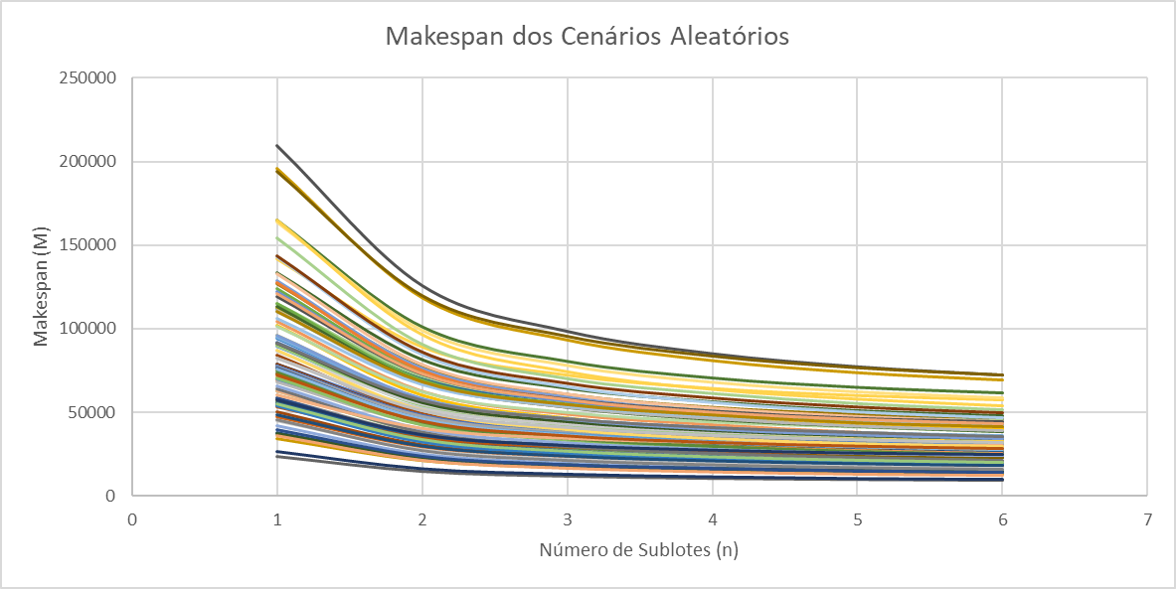
\includegraphics[width=12cm]{Resultados/Figuras/M05_50}
    \caption{Makespan dos cenários com 5 máquinas e variação de até 50\%}
    \label{fig:M05_50}
\end{figure}
    
    \begin{figure}[!ht]
    \centering
    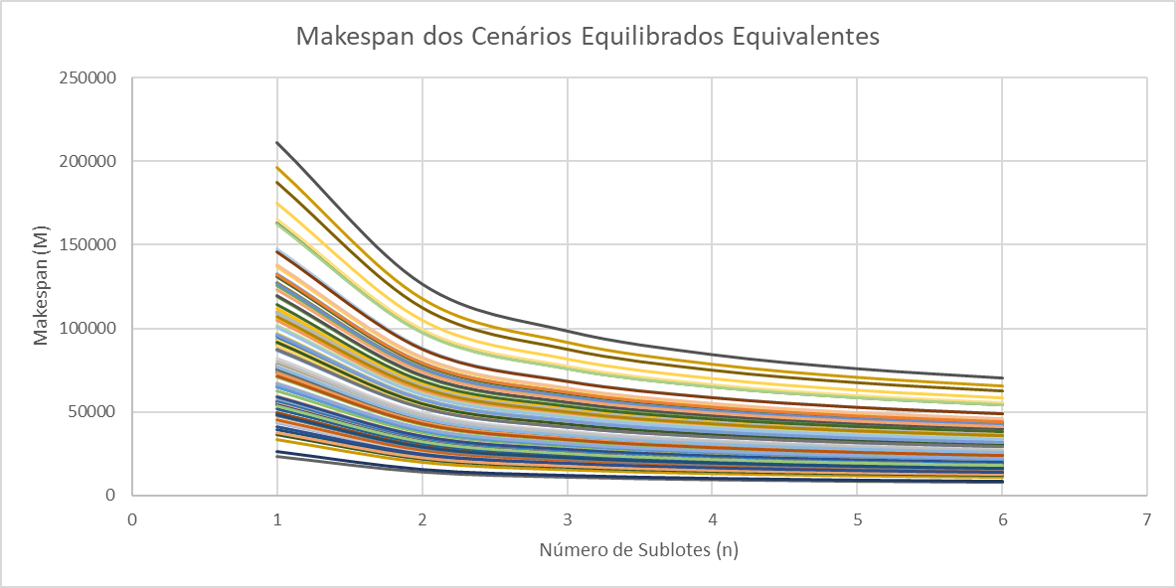
\includegraphics[width=12cm]{Resultados/Figuras/Meq05_50}
    \caption{Makespan dos cenários equilibrados equivalentes com 5 máquinas e variação de até 50\%}
    \label{fig:Meq05_50}
\end{figure}
    
    \begin{figure}[!ht]
    \centering
    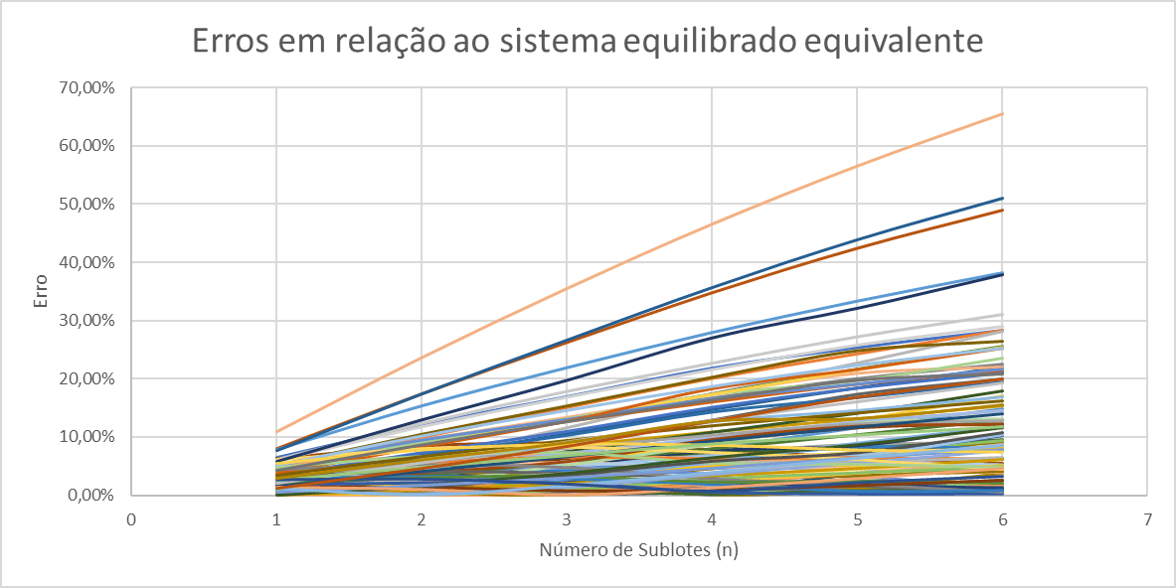
\includegraphics[width=12cm]{Resultados/Figuras/e05_50}
    \caption{Erros dos cenários com 5 máquinas e variação de até 50\%}
    \label{fig:e05_50}
\end{figure}
    
    Continuando nos conjuntos com 5 máquinas, porém este com variação de até 70\% representa sistemas de produção extremamente desequilibrados a fim de poder comparar futuramente com os cenários menos desequilibrados. As Figuras~\ref{fig:M05_70} e~\ref{fig:Meq05_70} representam conforme os anteriores, a evolução do \textit{Makespan} dos cenários e seus equivalentes, respectivamente. As comparações mais detalhadas encontram-se no Apêndice~\ref{app:fig05machine70} contendo as Figuras~\ref{fig:05m70_01-10} a~\ref{fig:05m70_91-100}. Nesse cenário mais desequilibrado já é possível notar que os erros são bem maiores que os anteriores (Figura~\ref{fig:e05_70}), sendo melhor explanado no tópico das análises.
    
    %% 5 Machine 70%
    \begin{figure}[!ht]
    \centering
    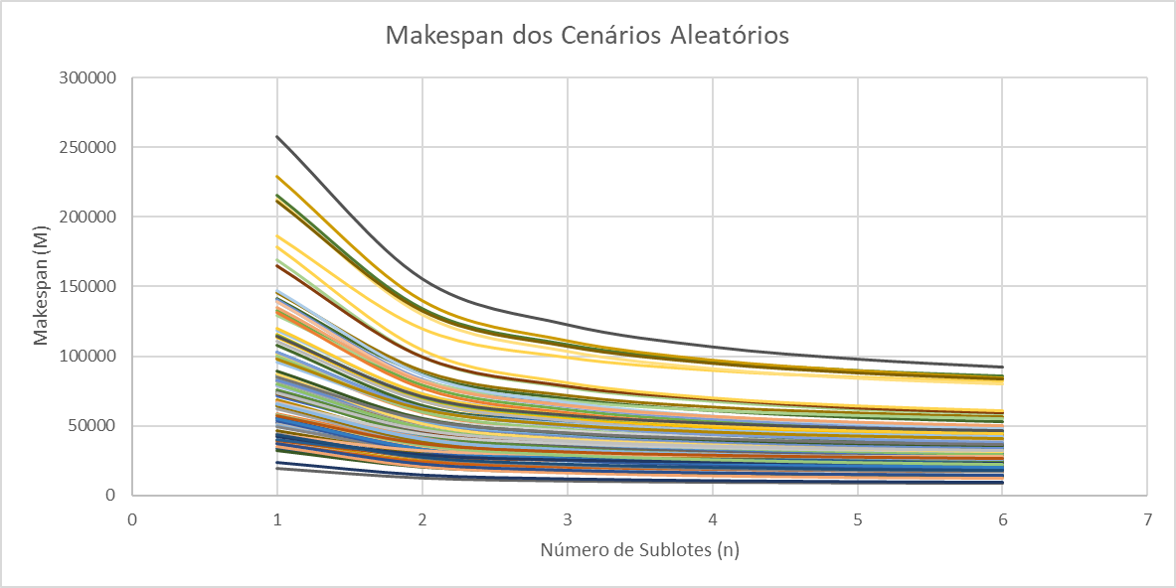
\includegraphics[width=12cm]{Resultados/Figuras/M05_70}
    \caption{Makespan dos cenários com 5 máquinas e variação de até 70\%}
    \label{fig:M05_70}
\end{figure}
    
    \begin{figure}[!ht]
    \centering
    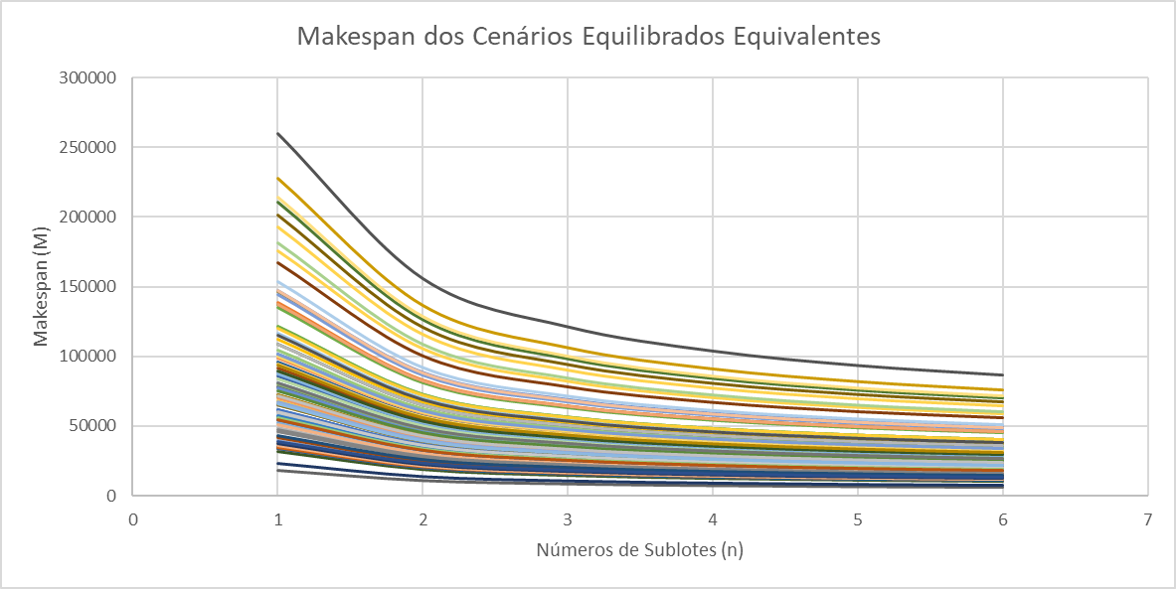
\includegraphics[width=12cm]{Resultados/Figuras/Meq05_70}
    \caption{Makespan dos cenários equilibrados equivalentes com 5 máquinas e variação de até 70\%}
    \label{fig:Meq05_70}
\end{figure}
    
    \begin{figure}[!ht]
    \centering
    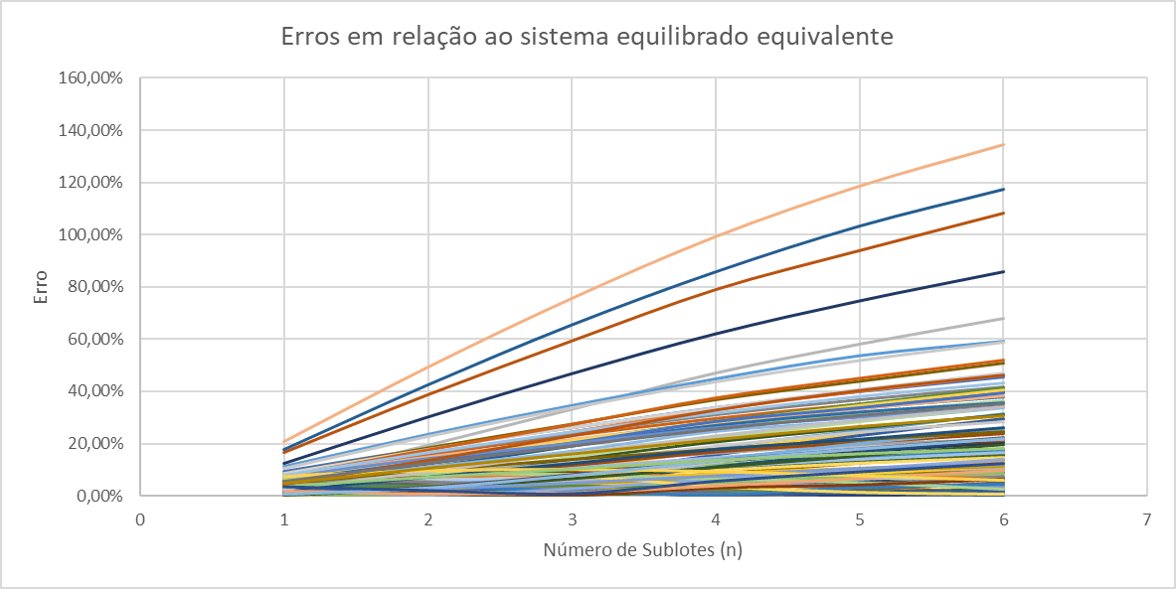
\includegraphics[width=12cm]{Resultados/Figuras/e05_70}
    \caption{Erros dos cenários com 5 máquinas e variação de até 70\%}
    \label{fig:e05_70}
\end{figure}
    
    Partindo para os cenários com 10 máquinas, primeiramente com variação de até 20\% nos tempos de máquinas. As Figuras~\ref{fig:M10_20} e~\ref{fig:Meq10_20} representam o \textit{Makespan} dos cenários desequilibrados bem como os equilibrados referentes a este conjunto, na ordem. Os erros podem ser vistos na Figura~\ref{fig:e10_20}. No Apêndice~\ref{app:fig10machine20} com as Figuras de~\ref{fig:10m20_01-10} a~\ref{fig:10m20_91-100} estão representados os seus cenários juntos, conforme os anteriores.
    
    %% 10 Machine 20%
    \begin{figure}[!ht]
    \centering
    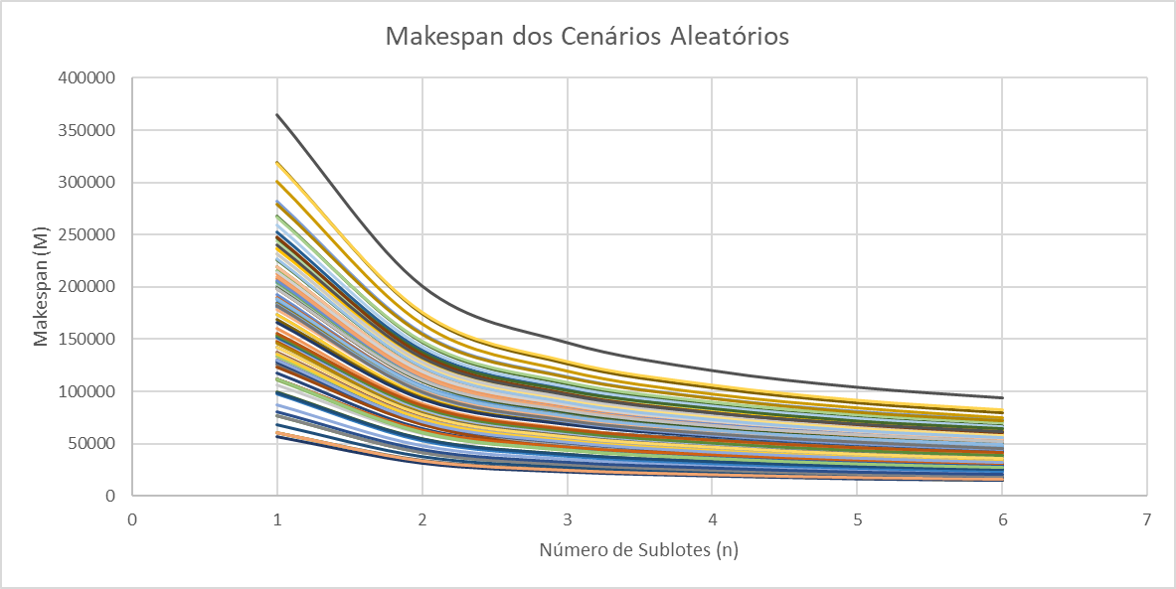
\includegraphics[width=12cm]{Resultados/Figuras/M10_20}
    \caption{Makespan dos cenários com 10 máquinas e variação de até 20\%}
    \label{fig:M10_20}
\end{figure}
    
    \begin{figure}[!ht]
    \centering
    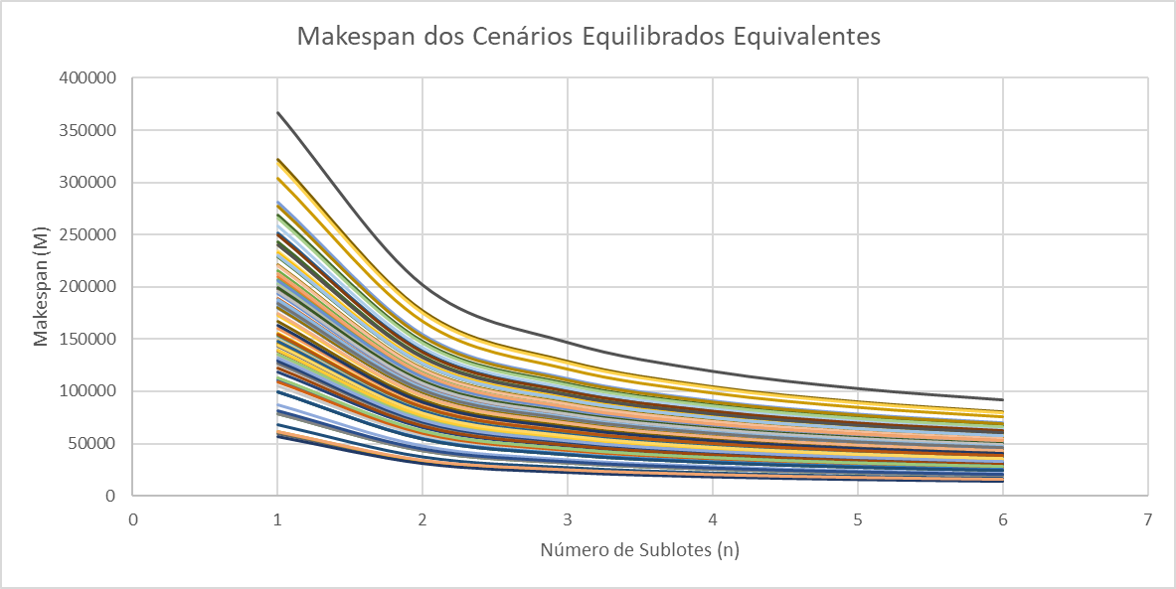
\includegraphics[width=12cm]{Resultados/Figuras/Meq10_20}
    \caption{Makespan dos cenários equilibrados equivalentes com 10 máquinas e variação de até 20\%}
    \label{fig:Meq10_20}
\end{figure}
    
    \begin{figure}[!ht]
    \centering
    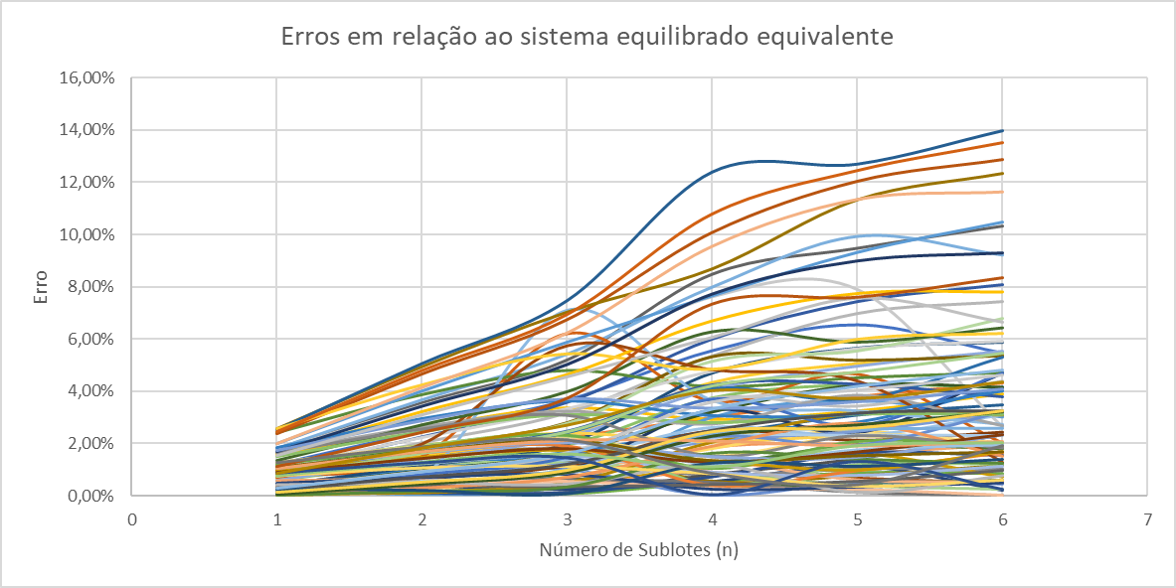
\includegraphics[width=12cm]{Resultados/Figuras/e10_20}
    \caption{Erros dos cenários com 10 máquinas e variação de até 20\%}
    \label{fig:e10_20}
\end{figure}
    
    Seguindo para os cenários com 10 máquina e, agora, 50\% de variação tem-se as Figuras~\ref{fig:M10_50} e~\ref{fig:Meq10_50} representando os \textit{Makespan} dos cenários desequilibrados e equilibrados, respectivamente, e a Figura~\ref{fig:e10_50} representando os erros gerados pelos resultados gerados deste conjunto. No Apêndice~\ref{app:fig10machine50} encontram-se os cenários mais detalhados (Figuras~\ref{fig:10m50_01-10} a~\ref{fig:10m50_91-100}).
    
    %% 10 Machine 50%
    \begin{figure}[!ht]
    \centering
    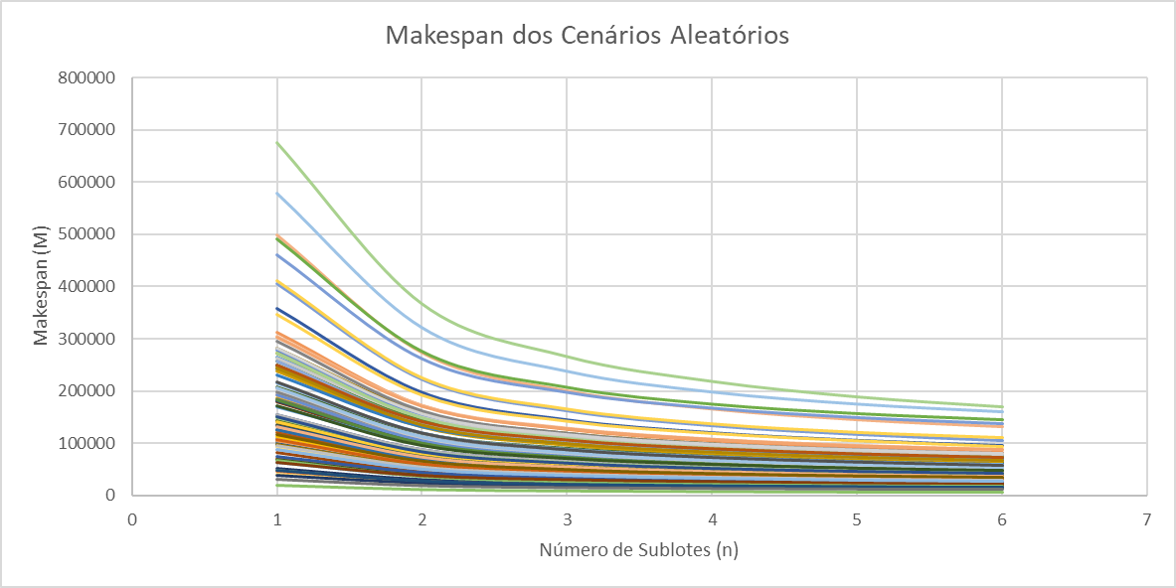
\includegraphics[width=12cm]{Resultados/Figuras/M10_50}
    \caption{Makespan dos cenários com 10 máquinas e variação de até 50\%}
    \label{fig:M10_50}
\end{figure}
    
    \begin{figure}[!ht]
    \centering
    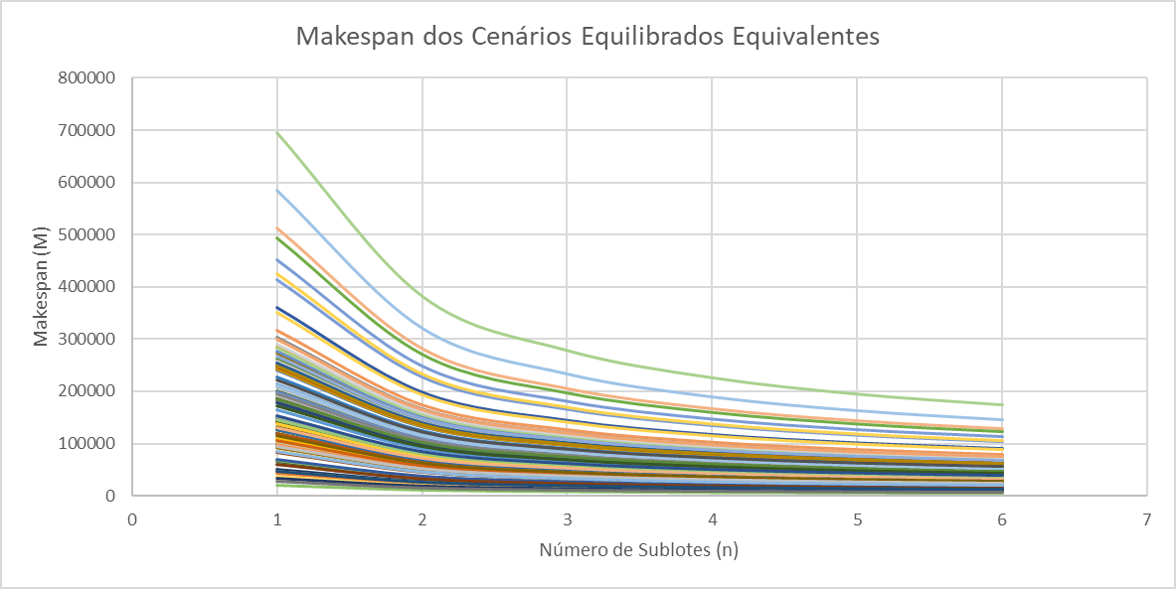
\includegraphics[width=12cm]{Resultados/Figuras/Meq10_50}
    \caption{Makespan dos cenários equilibrados equivalentes com 10 máquinas e variação de até 50\%}
    \label{fig:Meq10_50}
\end{figure}
    
    \begin{figure}[!ht]
    \centering
    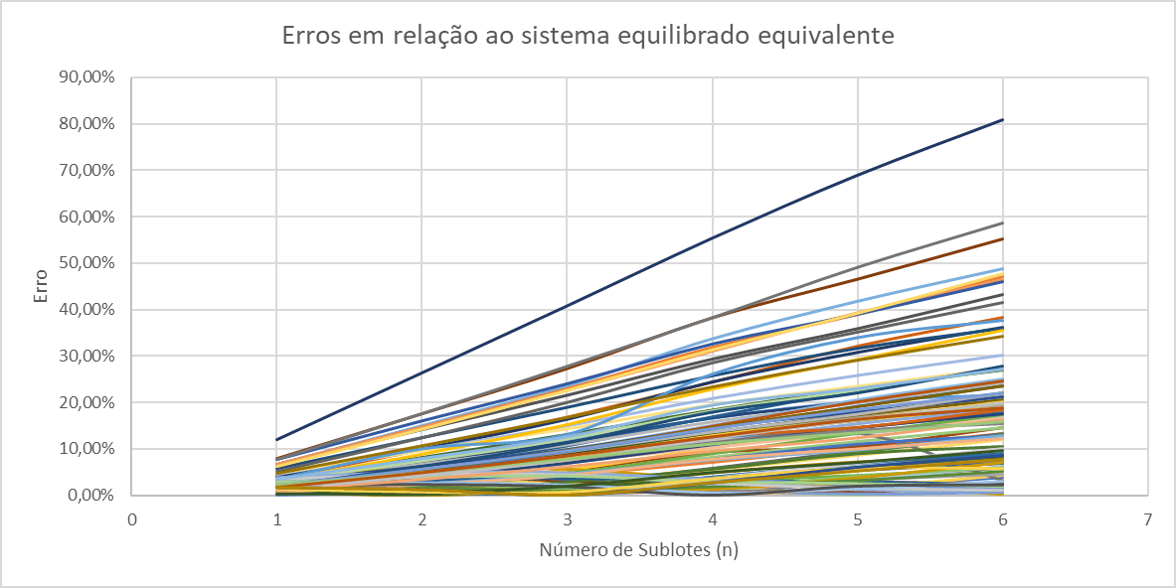
\includegraphics[width=12cm]{Resultados/Figuras/e10_50}
    \caption{Erros dos cenários com 10 máquinas e variação de até 50\%}
    \label{fig:e10_50}
\end{figure}
    
    Para o conjunto dos cenários com 10 máquinas e 70\% de variação apresenta-se a Figura~\ref{fig:M10_70} para o \textit{Makespan} dos cenários aleatórios desequilibrados, e a Figura~\ref{fig:Meq10_70} para seus equivalentes equilibrados, no Apêndice~\ref{app:fig10machine70} com as Figuras~\ref{fig:10m70_01-10} a~\ref{fig:10m70_91-100} apresentam os cenários detalhados. Os erros gerados pela diferença dos \textit{Makespan} é apresentada no gráfico da Figura~\ref{fig:e10_70}.
    
    %% 10 Machine 70%
    \begin{figure}[!ht]
    \centering
    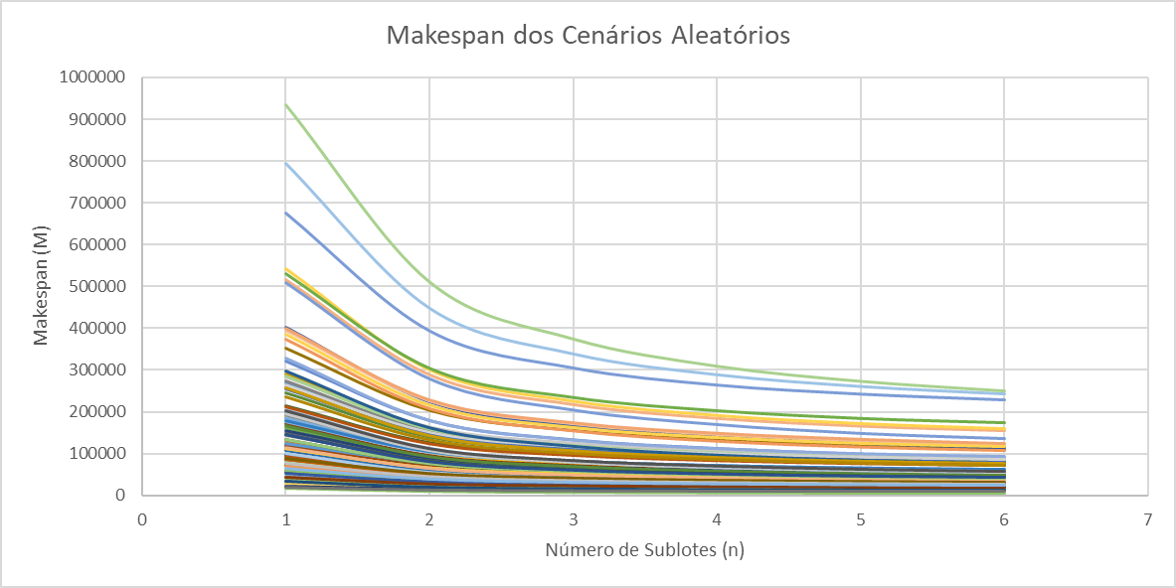
\includegraphics[width=12cm]{Resultados/Figuras/M10_70}
    \caption{Makespan dos cenários com 10 máquinas e variação de até 70\%}
    \label{fig:M10_70}
\end{figure}
    
    \begin{figure}[!ht]
    \centering
    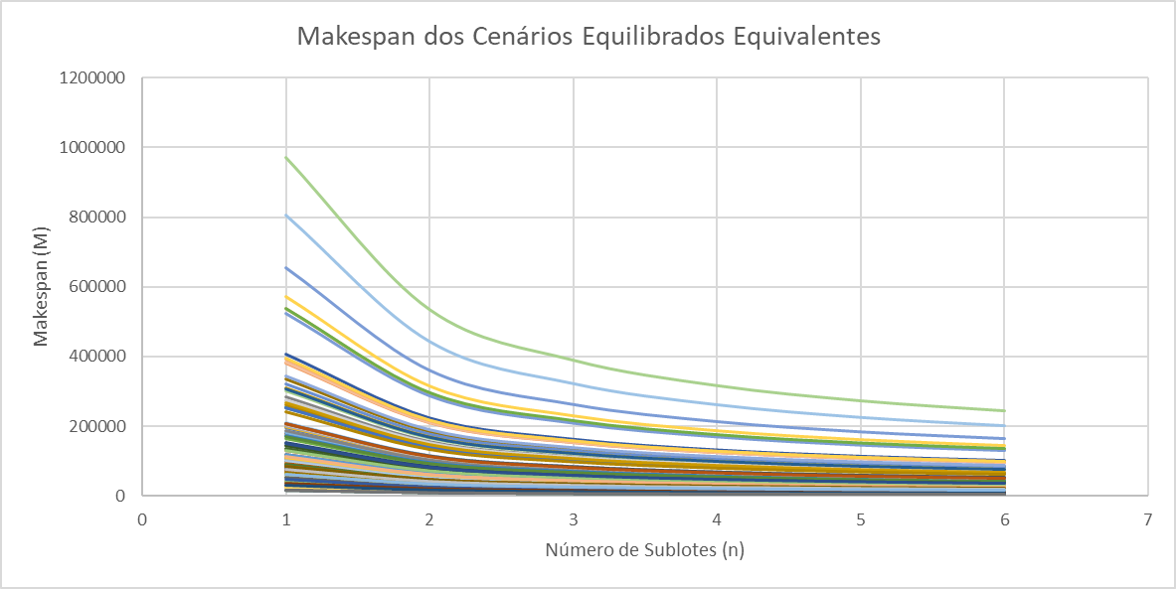
\includegraphics[width=12cm]{Resultados/Figuras/Meq10_70}
    \caption{Makespan dos cenários equilibrados equivalentes com 10 máquinas e variação de até 70\%}
    \label{fig:Meq10_70}
\end{figure}
    
    \begin{figure}[!ht]
    \centering
    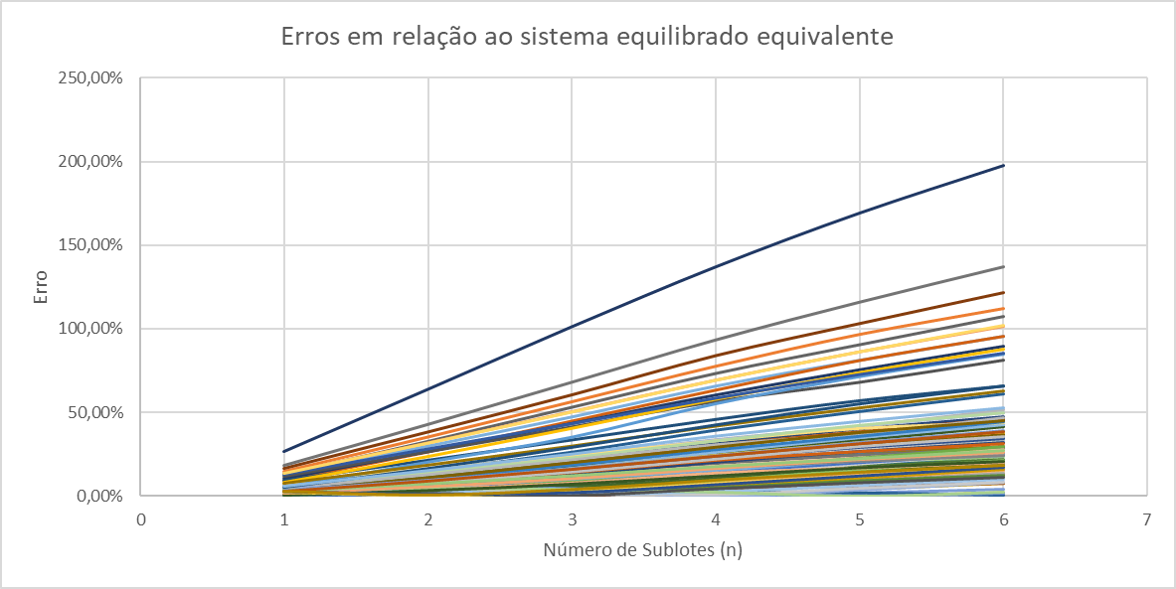
\includegraphics[width=12cm]{Resultados/Figuras/e10_70}
    \caption{Erros dos cenários com 10 máquinas e variação de até 70\%}
    \label{fig:e10_70}
\end{figure}
    
    De maneira semelhante, o conjunto de cenários com 15 máquinas e 20\% de variação é representado pelas Figuras~\ref{fig:M15_20},~\ref{fig:Meq15_20} e~\ref{fig:e15_20}, sendo a primeira o \textit{Makespan} dos cenários gerados aleatoriamente, em seguida dos resultados dos cenários equilibrados equivalente e por último os erros entre os resultados dos citados dois primeiros. Ainda, encontram-se no Apêndice~\ref{app:fig15machine20} os gráficos com as comparações mais detalhadas representados pelas Figuras~\ref{fig:15m20_01-10} a~\ref{fig:15m20_91-100}.
    
    %% 15 Machine 20%
    \begin{figure}[!ht]
    \centering
    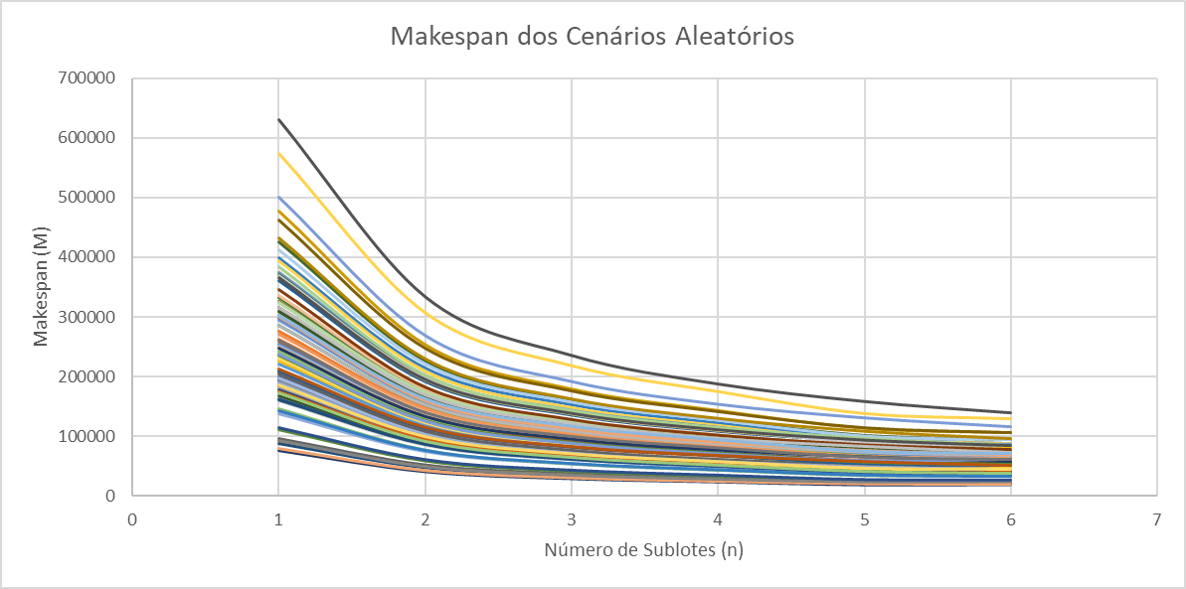
\includegraphics[width=12cm]{Resultados/Figuras/M15_20}
    \caption{Makespan dos cenários com 15 máquinas e variação de até 20\%}
    \label{fig:M15_20}
\end{figure}
    
    \begin{figure}[!ht]
    \centering
    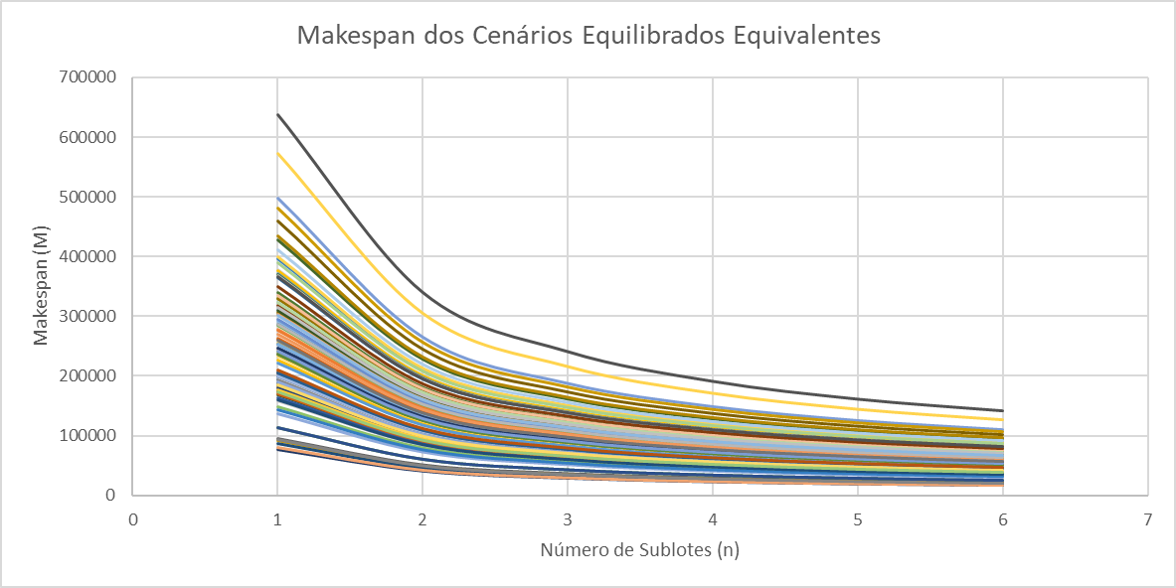
\includegraphics[width=12cm]{Resultados/Figuras/Meq15_20}
    \caption{Makespan dos cenários equilibrados equivalentes com 15 máquinas e variação de até 20\%}
    \label{fig:Meq15_20}
\end{figure}
    
    \begin{figure}[!ht]
    \centering
    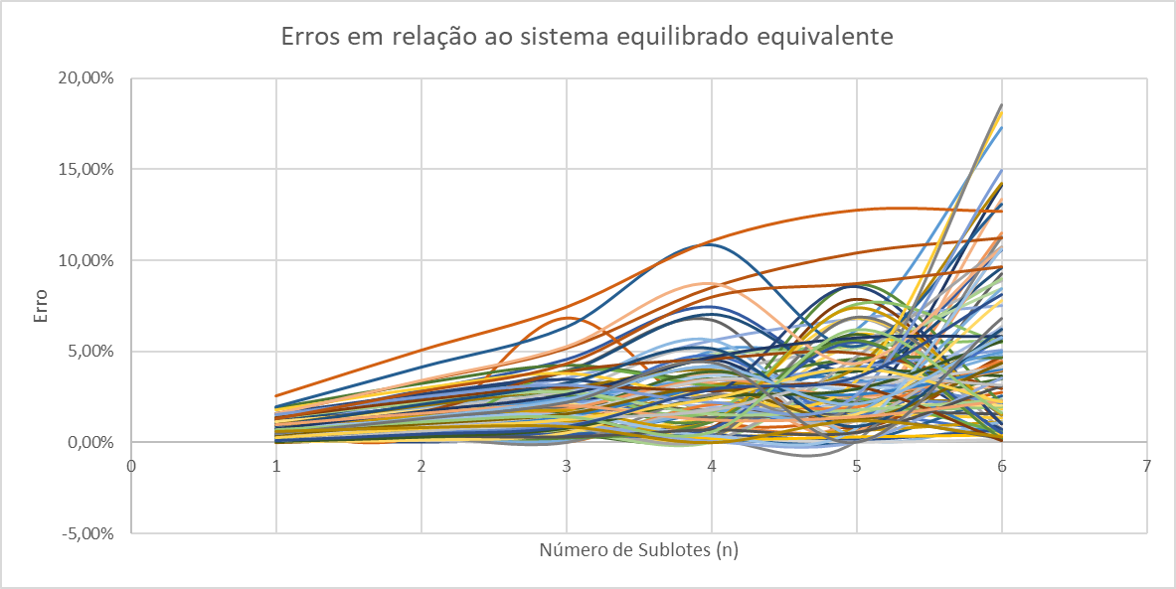
\includegraphics[width=12cm]{Resultados/Figuras/e15_20}
    \caption{Erros dos cenários com 15 máquinas e variação de até 20\%}
    \label{fig:e15_20}
\end{figure}
    
    O penúltimo conjunto simulado foi com cenários de 15 máquinas com variação de até 50\% entre máquinas consecutivas. Seguindo a mesma organização apresentada anteriormente estão dispostos o \textit{Makespan} dos cenários aleatórios desequilibrados (Figura~\ref{fig:M15_50}), o \textit{Makespan} dos cenários equilibrados (Figura~\ref{fig:M15_70}), e os erros calculados a partir da comparação dos cenários (Figura~\ref{fig:e15_50}). No Apêndice~\ref{app:fig15machine50} estão também as comparações dos cenário de 10 em 10 (Figuras~\ref{fig:15m50_01-10} a~\ref{fig:15m50_91-100}).
    
    %% 15 Machine 50%
    \begin{figure}[!ht]
    \centering
    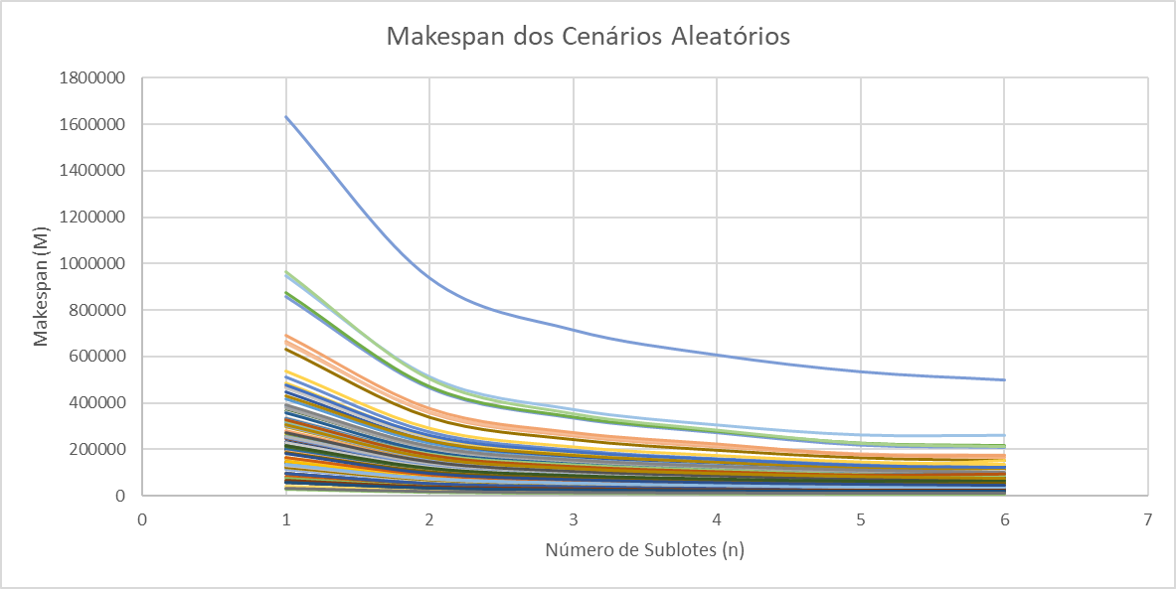
\includegraphics[width=12cm]{Resultados/Figuras/M15_50}
    \caption{Makespan dos cenários com 15 máquinas e variação de até 50\%}
    \label{fig:M15_50}
\end{figure}
    
    \begin{figure}[!ht]
    \centering
    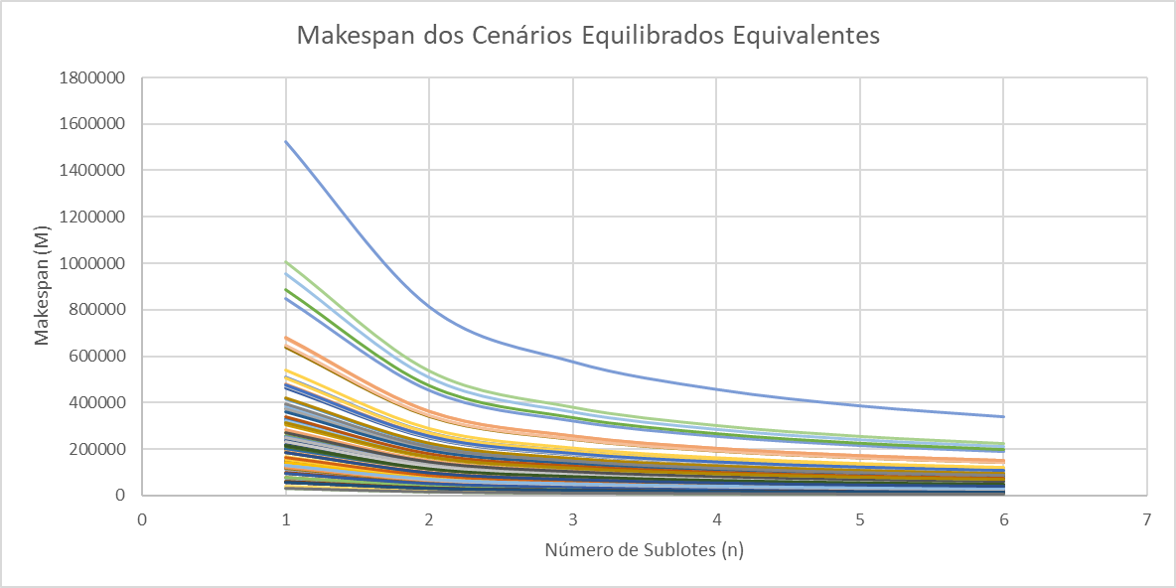
\includegraphics[width=12cm]{Resultados/Figuras/Meq15_50}
    \caption{Makespan dos cenários equilibrados equivalentes com 15 máquinas e variação de até 50\%}
    \label{fig:Meq15_50}
\end{figure}
    
    \begin{figure}[!ht]
    \centering
    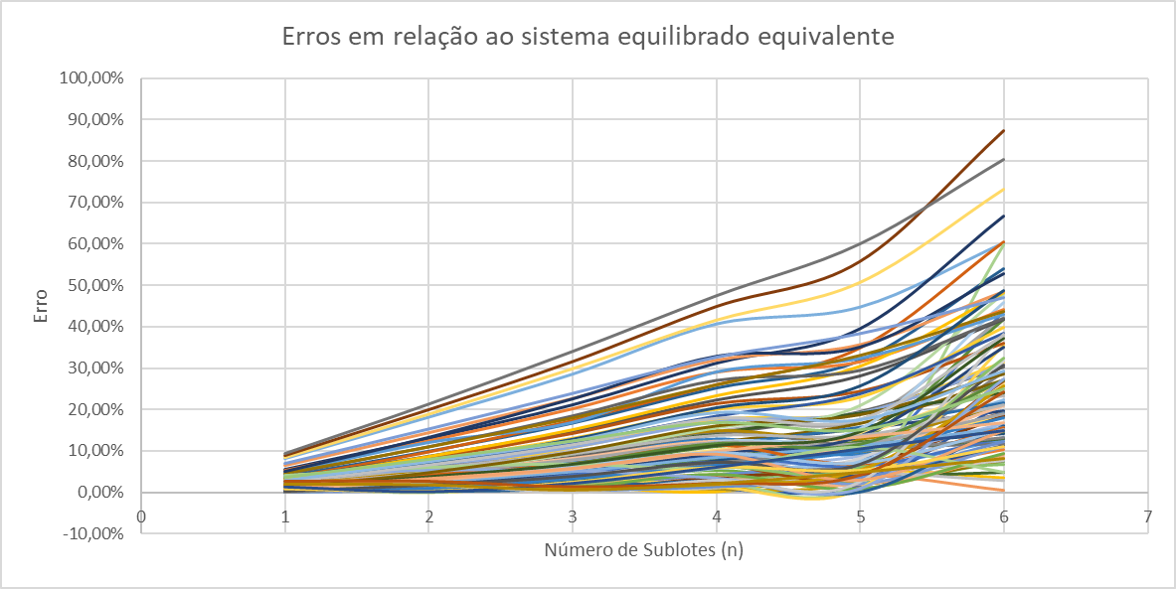
\includegraphics[width=12cm]{Resultados/Figuras/e15_50}
    \caption{Erros dos cenários com 15 máquinas e variação de até 50\%}
    \label{fig:e15_50}
\end{figure}
    
    Por fim, o conjunto de cenários com 15 máquinas e 70\% de variação. Conforme vem sendo feito, estão apresentados em ordem: o \textit{Makespan} dos cenários aleatórios (Figura~\ref{fig:M15_70}); o \textit{Makespan} dos cenários equilibrados equivalentes (Figura~\ref{fig:Meq15_70}; e os erros dos cenários analisados (Figura~\ref{fig:e15_70}). No Apêndice~\ref{app:fig15machine70} estão os cenários comparados com seus equivalentes, de maneira a melhor visualização de cada um, vide Figuras~\ref{fig:15m70_01-10} a~\ref{fig:15m70_91-100}.
    
    %% 15 Machine 70%
    \begin{figure}[!ht]
    \centering
    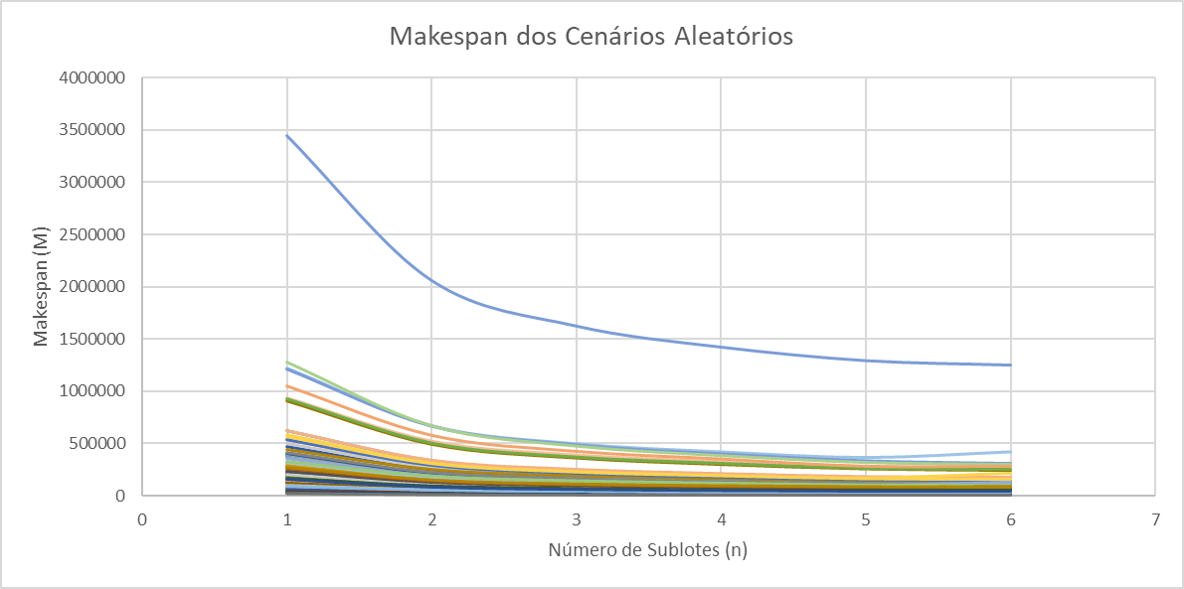
\includegraphics[width=12cm]{Resultados/Figuras/M15_70}
    \caption{Makespan dos cenários com 15 máquinas e variação de até 70\%}
    \label{fig:M15_70}
\end{figure}
    
    \begin{figure}[!ht]
    \centering
    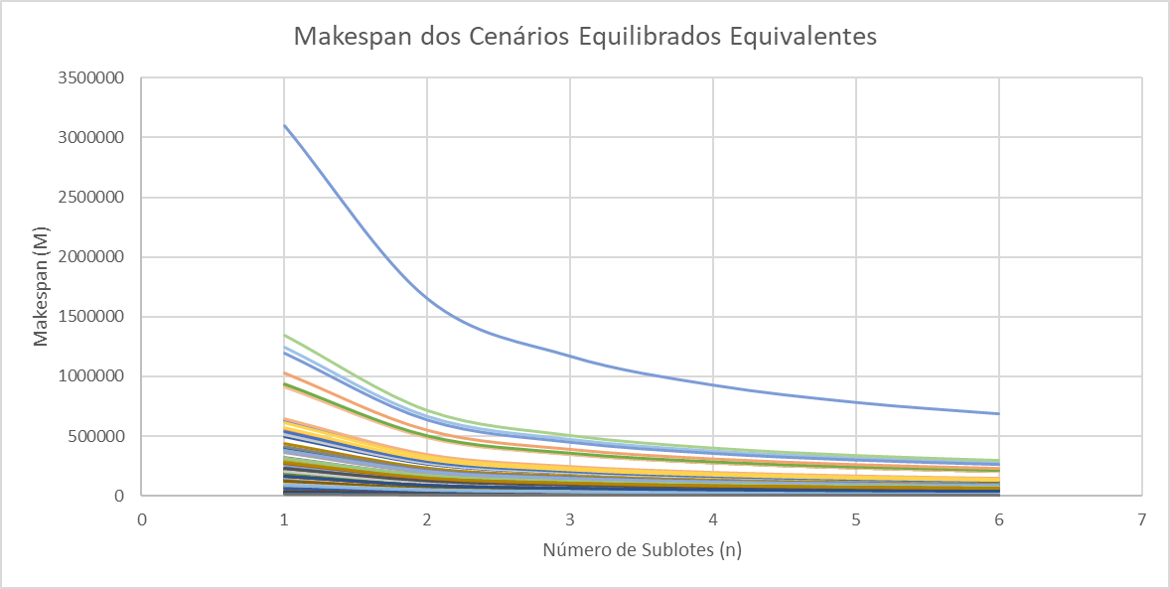
\includegraphics[width=12cm]{Resultados/Figuras/Meq15_70}
    \caption{Makespan dos cenários equilibrados equivalentes com 15 máquinas e variação de até 70\%}
    \label{fig:Meq15_70}
\end{figure}
    
    \begin{figure}[!ht]
    \centering
    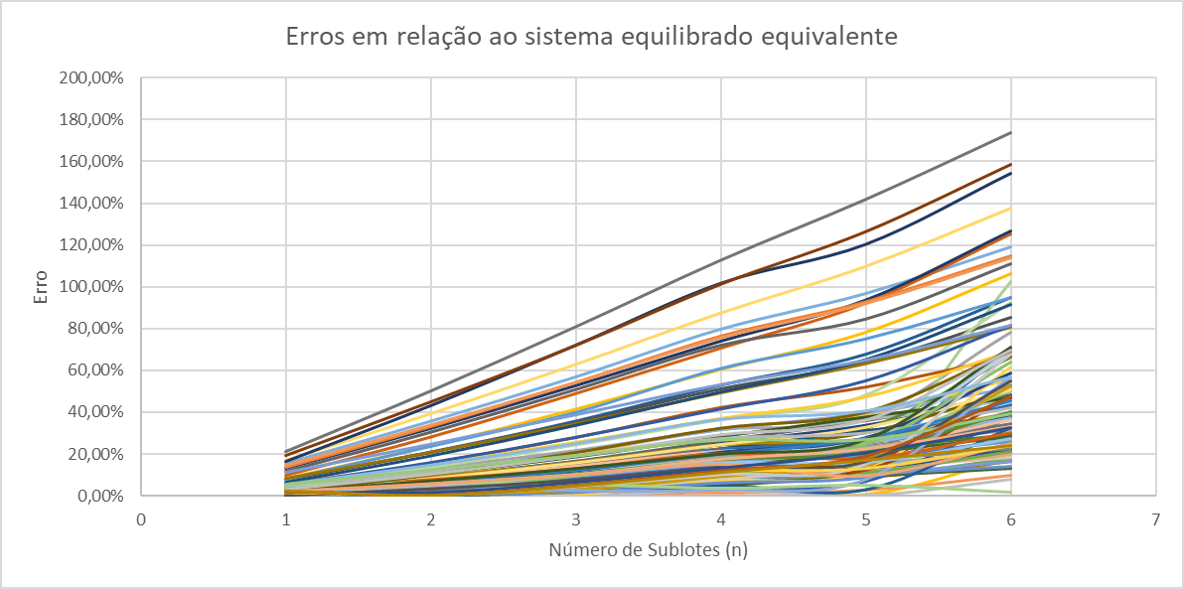
\includegraphics[width=12cm]{Resultados/Figuras/e15_70}
    \caption{Erros dos cenários com 15 máquinas e variação de até 70\%}
    \label{fig:e15_70}
\end{figure}
    
    %\FloatBarrier
    \subsubsection{Análise dos resultados}
    
    A partir dos resultados gerados pode-se portanto realizar algumas análises dos dados, principalmente pelos gráficos gerados. 
    
    Notou-se que em todos os cenários calculados, tanto os desbalanceados quanto os equilibrados que ele se comportam como uma assíntota decrescente, mostrando que o modelo está de acordo com a teoria das técnicas de \textit{Lot Streaming} já previa que isso ocorresse, corroborando portanto para a confiabilidade do modelo aplicado. 
    
    Ainda, é fato conhecido na Engenharia de Produção de que sistemas desequilibrados geralmente são mais ineficientes quando comparados à sistemas equilibrados. Nos resultados alcançados é possível ver claramente que os erros tendem a aumentar substancialmente conforme a variação dos tempos das máquinas aumenta. 
    
    Na Tabela~\ref{tab:resumoresults} foram apresentados os erros que tiveram mais frequência de cenários, bem como o erro máximo. No primeiro grupo de cenários (5 máquinas e variação de 20\%) a maior parte dos erros se mantiveram em até 6\%, com erro máximo de 13\%. Para variação de 50\%, os erros foram de até 30\% e erro máximo de 65\%. E com 5 máquinas e 70\% de variação, o maior parte dos erros foram de até 40\% e máximo de 135\%. Para o primeiro grupo de 10 máquinas, ou seja, com 20\% de variação nos tempos de máquinas, o erros mais frequentes também foram de até 6\% e máximo de 14\%. Já para 50\% de variação, o erro foi de até 30\% e máximo de 80\%. E para os cenários mais desequilibrados (com 70\% de variação), os erros se deram majoritariamente em até 50\% e com máximo que alcançou 200\%. Para o grupo com 15 máquinas, começando com variação de até 20\%, grande parte dos erros se mantiveram em até 8\% e apresentando um erro máximo de cerca de 18\%. Para variação de até 50\%, os erros foram sumariamente cerca de 50\% com máximo alcançado de 87\%. Por fim, nos cenários com 15 máquinas e variação de até 70\%, os erros se mantiveram majoritariamente em até 70\%, onde apresentou erro máximo de 175\%.
    
    % Please add the following required packages to your document preamble:
% \usepackage{multirow}
\begin{table}[!htb]
\caption{Resumo das análises dos erros gerados} \label{tab:resumoresults}
\begin{tabular}{>{\centering\arraybackslash}m{3cm} >{\centering\arraybackslash}m{4cm} >{\centering\arraybackslash}m{4cm} c}
\hline
Número de máquinas  & \% de variação dos tempos de processamento & Erro com maior frequência (\%) & Erro máximo (\%) \\ \hline
\multirow{3}{*}{5}  & 20                                         & 6                              & 13               \\
                    & 50                                         & 30                             & 65               \\
                    & 70                                         & 40                             & 135              \\ \hline
\multirow{3}{*}{10} & 20                                         & 6                              & 14               \\
                    & 50                                         & 30                             & 80               \\
                    & 70                                         & 50                             & 200              \\ \hline
\multirow{3}{*}{15} & 20                                         & 8                              & 18               \\
                    & 50                                         & 50                             & 87               \\
                    & 70                                         & 70                             & 175              \\ \hline
\end{tabular}
\end{table}
    
    Sistemas com variação de até 20\% em sua grande maioria apresentaram um erro de não mais que 8\%, ainda assim nos casos mais extremos o erro não ultrapassou 18\%. Nos cenários com a maior variação (de até 70\%), pode-se perceber o quanto os sistemas se distanciam do ideal, uma vez que no problema de 5 máquinas os erros se concentraram em até aproximadamente 40\%, no problema de 10 máquinas os erros foram em torno de 50\% apresentando também um cenário ao qual o máximo alcançou de 200\%, e para o problema de 15 máquinas a maior parte se manteve em até 70\%.
    
    Quanto mais se aumenta o número de máquinas, mais complexo o problema se torna, acrescentando a questão da aleatoriedade imposta na variação, percebe-se que os erros podem aumentar ainda mais. Mesmos nos casos com pouca variação, apenas com aumento no número de máquinas, os erros tenderam a crescer. Entretanto, os erros se mantiveram sempre em uma faixa de até 8\%, o que, dependendo do caso, pode não ser uma perda tão significativa na produção. 
    
    



%% APRESENTAR COMO É CALCULADO O LOT STREAMING, TANTO O CONTINUO QUANTO O DISCRETO
%% MOSTRAR COMO SE CALCULA OS CENÁRIOS EQUILIBRADOS

%% EXPLICAR QUE OS CENÁRIOS FORAM GERADOS A PARTIR DE MONTE CARLO, DEVIDO A QUANTIDADE DE SIMULAÇÕES
%% MOSTRAR COMO FOI GERADO OS CENÁRIOS E APRESENTAR QUAIS SÃO
%% MOSTRAR OS CENÁRIOS EQUILIBRADOS CALCULADOS

%% APRESENTAR OS RESULTADOS DE TODOS OS CENÁRIOS COM GRÁFICOS E TABELAS
%% APRESENTAR OS ERROS E COMO FORAM CALCULADOS A FIM DE VALIDAR A ESCOLHA DE UM SISTEMA TOTALMENTE EQUILIBRADO

%% POSSIVELMENTE AS TABELAS ESTARÃO EM ANEXO